
%=======================================================================
% React hoofdstuk
%=======================================================================

\chapter{\IfLanguageName{dutch}{React}{React}}
\label{ch:react}

React is een open source \gls{js}-library dat werd geïntroduceerd in 2013 door het development team van Facebook. Figuur~\ref{fig:reactTijdlijn} op pagina~\pageref{fig:reactTijdlijn} is een vereenvoudigde tijdlijn dat de evoluties van React aangeeft tot heden.\\ 
Vanuit het standpunt dat React een framework is, kan het geen volgend populair \gls{mvc} framework genoemd worden. Eerder is React vervanger voor de V binnen \gls{mvc}. Views in traditionele \gls{mvc}-frameworks zijn aanzien als logica loze files die worden aangestuurd door een controller.\\
React maakt gebruik van componenten voor het definiëren van speciaal op maat gemaakte \gls{html}-tags. Deze zijn een combinatie van \gls{html} en plain javaScript, waarbij elk component gedefinieerd wordt in een aparte file, wat een makkelijk leesbare structuur oplevert. Het is bedoeld om alle \gls{ui} elementen onder te verdelen in zo klein mogelijke componenten, zodat deze doorheen de codebase makkelijk hergebruikt kunnen worden. De \gls{ui} van een React applicatie wordt opgebouwd door alle componenten samen te voegen tot één geheel.\\

\begin{figure}[H]
    \tikz\node [drop shadow={
        shadow scale=0.98,
        shadow xshift=0ex,
        shadow yshift=0ex,
        opacity=0.2,
    }]
    {\fcolorbox{black}{white}{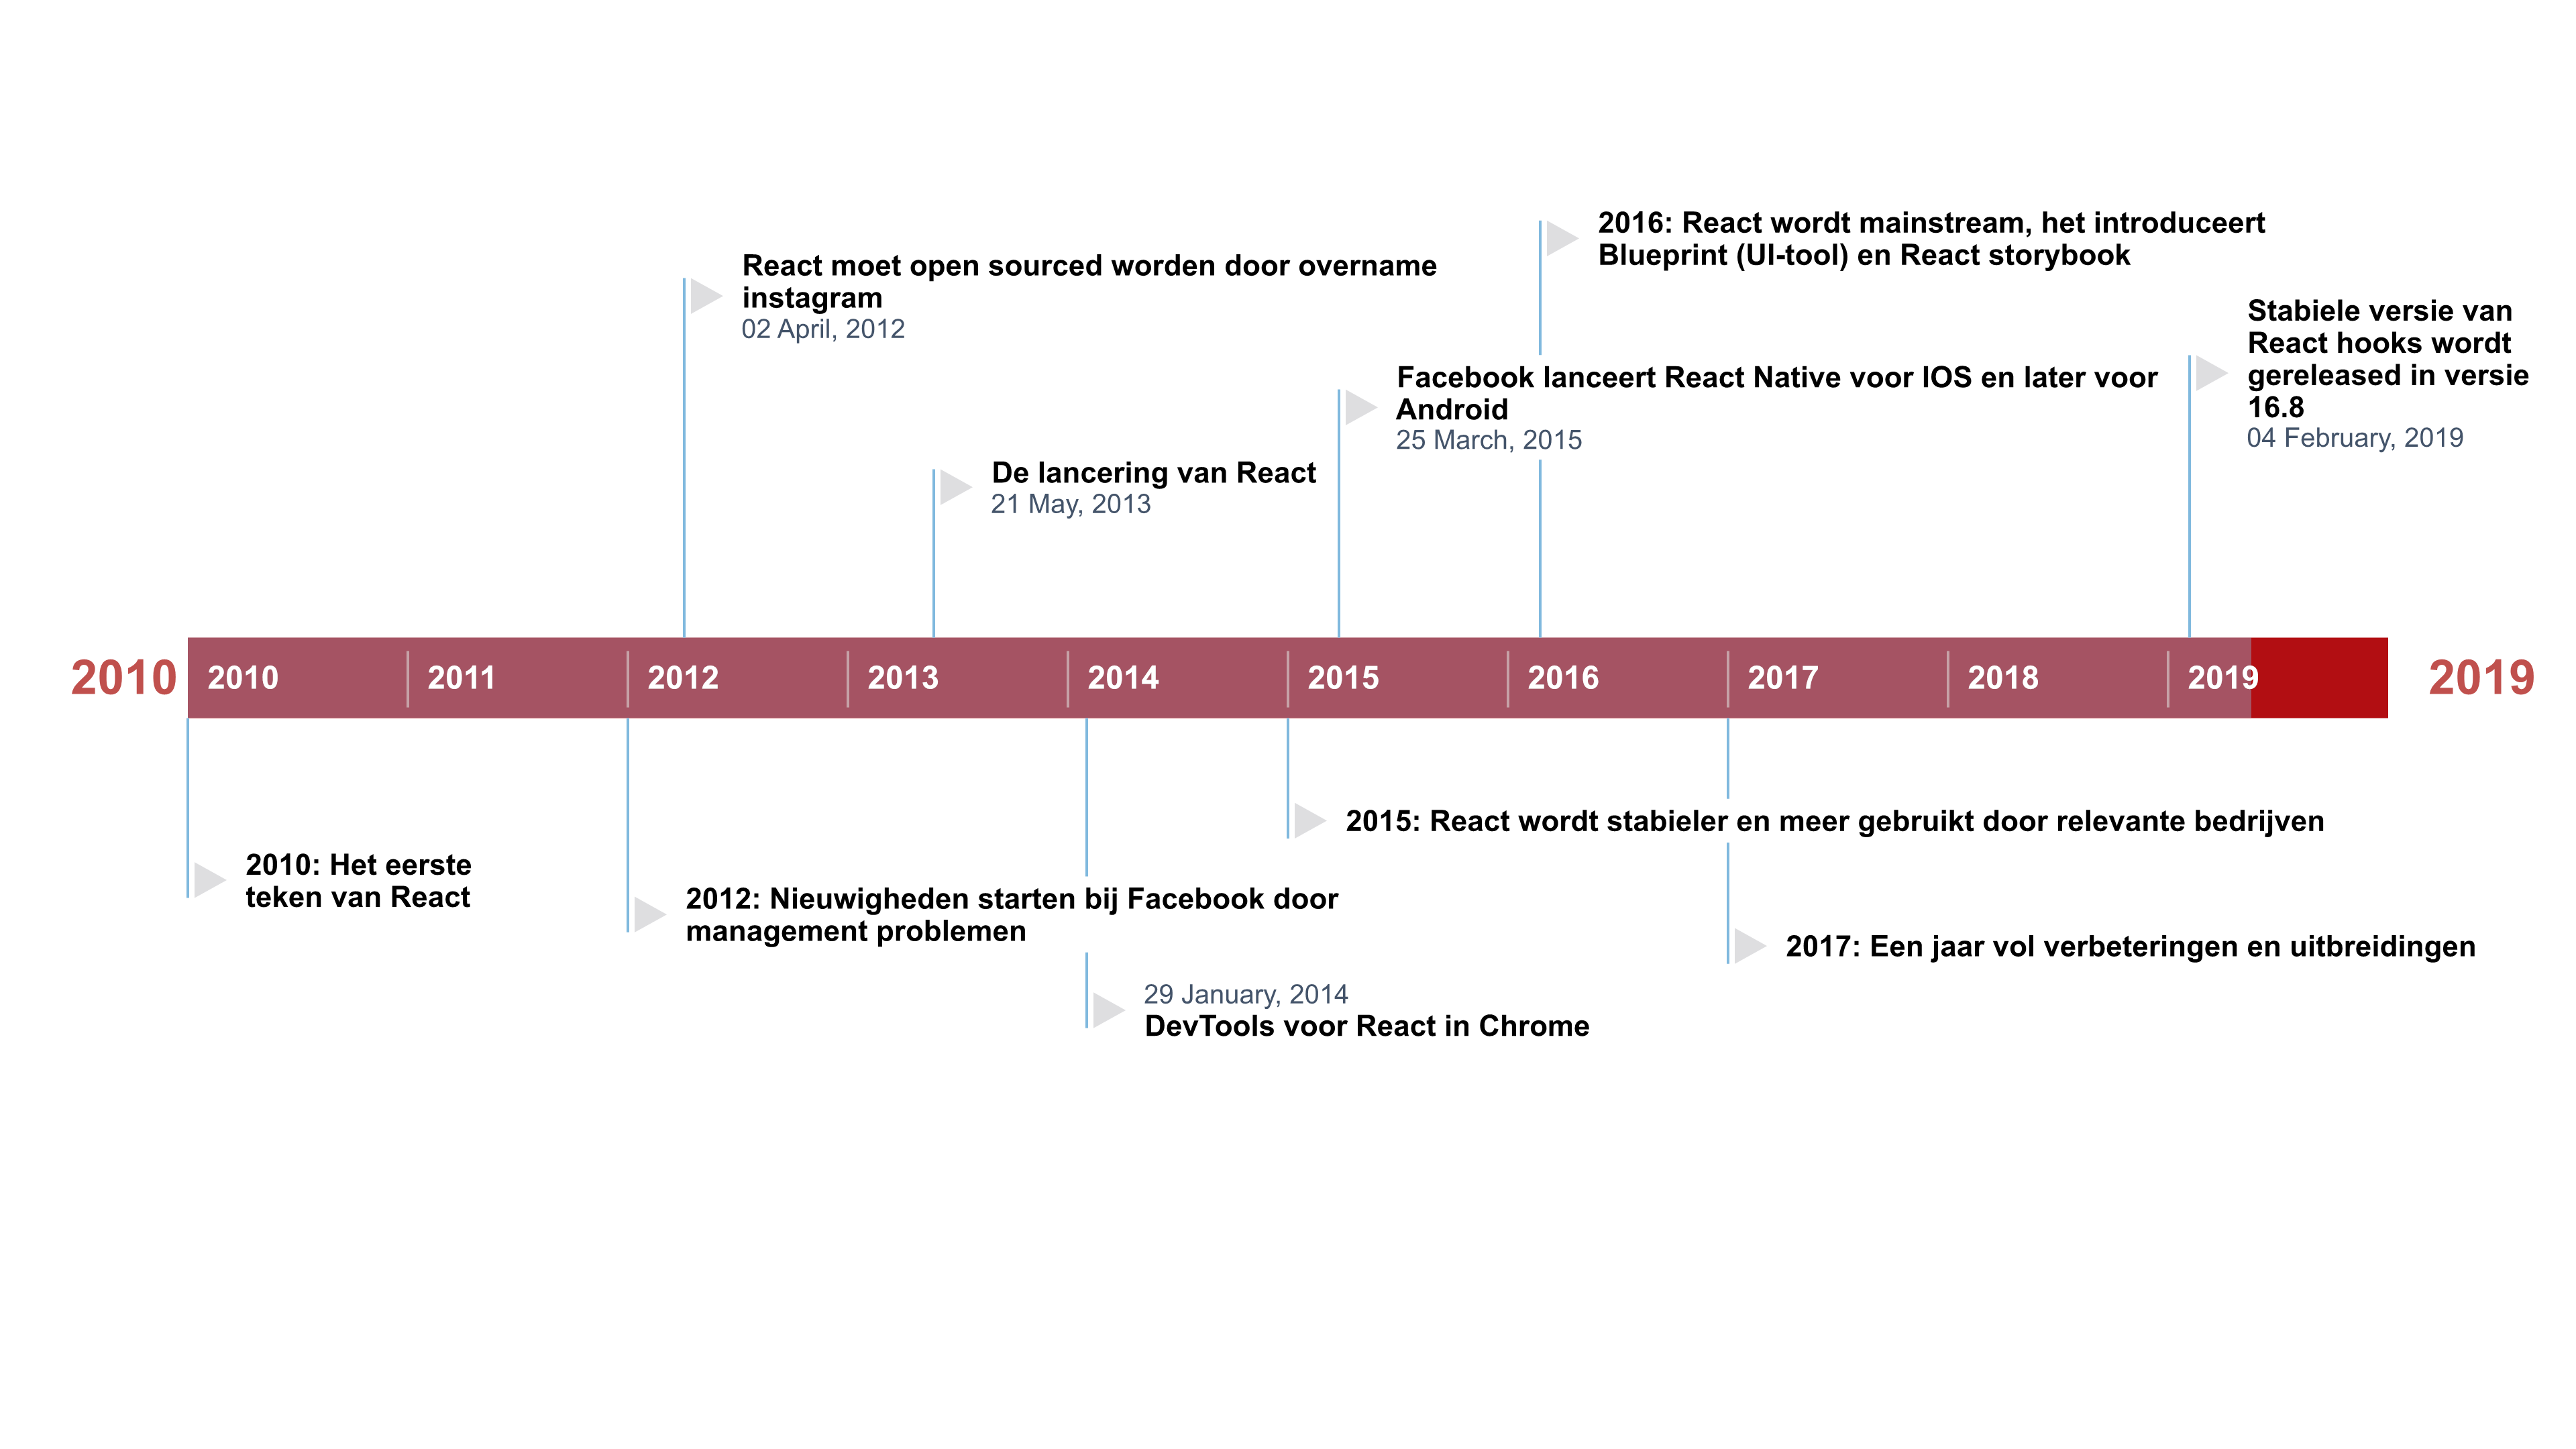
\includegraphics[width=\linewidth]{React_tijdlijn.png}}};
    \caption{Product tijdlijn React}
    \label{fig:reactTijdlijn}
\end{figure}

\section{\IfLanguageName{dutch}{JSX}{JSX}}
\label{sec:jsx}

De JavaScript eXtension (\gls{jsx}) wordt gebruikt voor het definiëren van React elementen in een \gls{html} formaat. De compiler vertaalt de \gls{jsx} code naar gewone javaScript tijdens runtime. \gls{jsx} geeft een virtuele \gls{html} visualisatie van hoe het component er in de \gls{dom} uitziet. Het is een vereenvoudigde presentatie van een nesting van React elementen die elk respectievelijk worden aangemaakt met `React.createElement()`. In \gls{jsx} wordt elk van die elementen voorgesteld in een \gls{html}-tag.\\
Zoals wordt aangetoond in Code fragment~\ref{fig:translatedJSX} op pagina~\pageref{fig:translatedJSX} is de syntax aanzienlijk eenvoudiger met \gls{jsx}.\\

\begin{lstlisting}[caption=JSX naar gewone javaScript, label={fig:translatedJSX}]
    // HelloComponent.js met JSX syntax
    export class HelloComponent extends React.Component {
        render () {
            return (
                <div>Hello world!</div>
            );
        }
    }
    
    // HelloComponent.js zonder JSX syntax
    export class HelloComponent extends React.Component {
        render () {
            return (
                React.createElement(
                    'div',
                    null {/* Properties van de HTML-tag zoals 'name', 'alt', ... */},
                    'Hello world!'
                )
            );
        }
    }
\end{lstlisting}

\section{\IfLanguageName{dutch}{Componenten}{Components}}
\label{sec:componenten}

Componenten zijn de bouwstenen voor een React \gls{ui}. Ze dienen om React elementen aan te maken die op hun beurt beschrijven hoe het specifieke deel van de \gls{ui} er moet uitzien. Optioneel kan er input meegegeven worden aan een component in de vorm van properties. Naast optionele input kunnen componenten ook een lokale state bijhouden waar waarden worden in opgeslagen. De waarden kunnen veranderen doorheen de levenscyclus van het component.\\
Er bestaan twee soorten, functionele en klasse componenten. Vóór React versie 16.8 was er een duidelijk verschil tussen de twee soorten en door de komst van React hooks in versie 16.8 is dit helemaal veranderd.

\subsection{\IfLanguageName{dutch}{Klasse componenten}{Class components}}
\label{sec:klasseComp}

Klasse componenten hebben dezelfde bouw als klassen in een object-georiënteerde programmeertaal zoals Java. Ze kunnen allebei erven van andere modules en bevatten functies en/of waarden die de inhoud kunnen veranderen. Het grote verschil tussen beiden zit in de methodologie. Bij klasse componenten wordt er altijd een specifiek deel van de \gls{ui} geretourneerd via een render functie en er kunnen waarden in een lokale state worden geplaatst die invloed hebben op de geretourneerde \gls{ui}. Ze bevatten lifecycle methoden die uitgevoerd worden doorheen de levenscyclus van een component, zoals de render, componentDidMount, componentWillMount,\dots functies.\\
In Code fragment~\ref{fig:classComponent} op pagina~\pageref{fig:classComponent} is een simpele representatie uitgeschreven van een klasse component.

\newpage
\begin{lstlisting}[caption=Een klasse component, label={fig:classComponent}]
    import React from 'react';
    import logo from '../logo.svg';
    
    // ListItem component als klasse component
    export class ListItem extends React.Component {
        render () {
            return (
                <ListItemContainer>
                    <LogoWrapper><Logo src={logo} alt="logo" /></LogoWrapper>
                    <ContentWrapper>
                        <h2>Dit is de titel van het item</h2>
                        <Paragraph>
                            Dit is waar de inhoud normaal komt, maar er is geen..
                        </Paragraph>
                    </ContentWrapper>
                </ListItemContainer>
            );
        }
    }
\end{lstlisting}

\subsection{\IfLanguageName{dutch}{Functionele componenten}{Functional components}}
\label{sec:funcComp}

Vóór React hooks werden functionele componenten gebruikt voor een beknopte presentatie te maken van React elementen. Ze kunnen optioneel input krijgen waarmee ze een bepaald deel van de \gls{ui} retourneren. Functionele componenten hadden geen logica en/of state waardoor ze heel voorspelbaar waren, dus werden deze componenten stateless genoemd. Code fragment~\ref{fig:functionalComponent} op pagina~\pageref{fig:functionalComponent} toont een stateless functioneel component.\\
Met de komst van React hooks kunnen functionele componenten statefull gemaakt worden en logica bevatten. De bruikbaarheid is naar het niveau van klasse componenten getrokken. Door de veranderingen is het mogelijk om meer overzichtelijke en makkelijk leesbare componenten te maken. In het boek van Robert C. Martin ~\autocite{Martin2008} wordt aangehaald waarom dit voordelig is:

\begin{quote}
    \textit{Indeed, the ratio of time spent reading versus writing is well over 10 to 1. We are constantly reading old code as part of the effort to write new code. ...[Therefore,] making it easy to read makes it easier to write.}
\end{quote}

\begin{lstlisting}[caption=Een functioneel component, label={fig:functionalComponent}]
    import React from 'react';
    import logo from '../logo.svg';
    
    // ListItem component als functioneel component
    export const ListItem = () => (
        <ListItemContainer>
            <LogoWrapper><Logo src={logo} alt="logo" /></LogoWrapper>
            <ContentWrapper>
                <h2>Dit is de titel van het item</h2>
                <Paragraph>
                    Dit is waar de inhoud normaal komt, maar er is geen..
                </Paragraph>
            </ContentWrapper>
        </ListItemContainer>
    );
\end{lstlisting}

\subsection{\IfLanguageName{dutch}{Componenten exporteren}{Exporting components}}
\label{sec:exportComp}

Componenten worden gemaakt in hun specifieke file en geïmporteerd in een andere om ze daar in scope te plaatsen en te gebruiken. Om een component te importeren in een file moet deze dus eerst geëxporteerd worden uit zijn eigen file.\\
Er zijn twee manieren om een component te exporteren. De klasse of functionele constante kan expliciet of impliciet geëxporteerd worden, dit is te zien in Code fragment~\ref{fig:exportComp} op pagina~\pageref{fig:exportComp}.\\
Bij expliciet exporteren wordt het component ook expliciet geïmporteerd onder die naam. Impliciet exporteren geeft de mogelijkheid om het component onder een ander naam te importeren. Een impliciete export kan enkel één keer per file gedaan worden.\\

\begin{lstlisting}[caption=Exporteren van een component, label={fig:exportComp}]
    //Expliciet exporteren en importeren van een klasse component
    export class HelloComponent extends React.Component {
        render () {
            return (
                <div>Hello world!</div>
            );
        }
    }
    
    import { HelloComponent } from './helloComponent.js';
    
    
    //Impliciet exporteren en importeren van een klasse component
    class HelloComponent extends React.Component {
        render () {
            return (
                <div>Hello world!</div>
            );
        }
    }
    export default HelloComponent;
    
    import HelloComponent from './helloComponent.js';
\end{lstlisting}


\section{\IfLanguageName{dutch}{Fragments}{Fragments}}
\label{sec:fragments}

Een React component retourneert altijd een (klein) deel van de \gls{ui}. Hetgeen dat wordt geretourneerd is een nesting van React elementen die samen gebonden zijn in één ouder element. Fragments voorkomen de vervuiling van het \gls{dom} met nutteloze omhullende ouder tags, voornamelijk <div> tags, die dienen voor het samenbinden van React elementen. De fragment tag retourneert al zijn kinderen zonder aanvullende \gls{html}-tags, dus is er minder vervuiling van het \gls{dom} en voorkomt men het overvloedig nesten van elementen.\\
In Code fragment~\ref{fig:fragments} op pagina~\pageref{fig:fragments} wordt een onderscheid gemaakt tussen het gebruik zonder en met fragment tag.

\newpage
\begin{lstlisting}[caption=Gebruik van de Fragment tag, label={fig:fragments}]
    // HelloComponent.js zonder Fragment als ouder tag
    import React from 'react';
    
    export class HelloComponent extends React.Component {
        render () {
            return (
                <div>
                    <div>Hallo,<div>
                    <div>Groetjes aan iedereen!</div>
                </div>
            );
        }
    }
    
    // HelloComponent.js met Fragment als ouder tag
    import React from 'react';
    
    export class HelloComponent extends React.Component {
        render () {
            return (
                <React.Fragment>
                    <div>Hallo,<div>
                    <div>Groetjes aan iedereen!</div>
                </React.Fragment>
            );
        }
    }
\end{lstlisting}

\section{\IfLanguageName{dutch}{Props}{Props}}
\label{sec:properties}

De properties, of props genaamd, van een component zijn een gewoon javaScript object die alle input waarden bevat die aan de component worden meegegeven. Het meegeven van props aan een component zorgt ervoor dat deze dynamisch aan te maken zijn. De props bepalen hoe het te retourneren deel van de \gls{ui} er zal uitzien. Ze zorgen ervoor dat er data kan worden doorgegeven naar andere componenten, dit in de meeste gevallen van een ouder naar zijn kind. Deze toepassing zorgt ervoor dat de unidirectional data flow, waar React op steunt, wordt behouden.\\
Props zijn bovendien read-only, wat wil zeggen dat ze niet aanpasbaar zijn doorheen de levenscyclus van een component. Wanneer data moet veranderen tijdens de levenscyclus van een component gebruiken we state.

\subsection{\IfLanguageName{dutch}{Prop types}{Prop types}}
\label{sec:propTypes}

Het is een best practice om voor alle componenten de data die binnen komt te definiëren. Door het expliciet definiëren wordt het duidelijk wat componenten verwachten om goed te kunnen functioneren.

\subsection{\IfLanguageName{dutch}{Default props}{Default props}}
\label{sec:defaultProps}

Wanneer een bepaalde property in de component visuele waarde heeft, is bij afwezigheid van die property een deel van de \gls{ui} onvolledig. Om dergelijke scenario's te vermijden stellen we een standaard waarde in voor properties die onvoorzien kunnen zijn. Door properties een standaard waarde te geven maken we de componenten veerkrachtig.\\

\begin{lstlisting}[caption=Functioneel component met properties, label={fig:componentWithProps}]
    import React from 'react';
    import PropTypes from 'prop-types';
    
    import logo from '../logo.svg';
    
    // ListItem component als klasse component
    export const ListItem = (props) => (                
        <ListItemContainer>
            <LogoWrapper><Logo src={logo} alt="logo" /></LogoWrapper>
            <ContentWrapper>
                <h2>{props.title}</h2>
                <Paragraph>{props.text}</Paragraph>
            </ContentWrapper>
        </ListItemContainer>
    );
    
    ListItem.defaultProps = {
        text: 'Er werd geen inhoud tekst meegegeven',
    }
    
    ListItem.defaultProps = {
        title: PropTypes.string.isRequired,
        text: PropTypes.string
    }
\end{lstlisting}

\section{\IfLanguageName{dutch}{State}{State}}
\label{sec:state}

State is, net zoals de properties, een javaScript object waar data wordt in opgeslagen. De data in de state kan doorheen de levenscyclus van een component veranderen door middel van `setState()`. Wanneer setState wordt aangeroepen gaat het volledige component worden herladen, ook wel rerender genaamd. Alle elementen in het component die de aangepaste data uit de state gebruiken gaan die nieuwe data invullen.\\
Binnen een component is state aanzien als immutable, wat wil zeggen dat de state niet rechtstreeks mag aangepast worden door gebruik te maken van `this.state`. Het aanpassen van de state met setState zorgt voor de immutability van de state. Bij componenten met een grote state is een goede benadering een kopie maken van het reeds bestaande state object, dit aan te passen en het nieuwe object mee te geven aan setState.\\
In Code fragment~\ref{fig:classCompWithProps&State} op pagina~\pageref{fig:classCompWithProps&State} is een statefull klasse component uitgewerkt die met setState de zijn interne state gaat aanpassen. Code fragment~\ref{fig:funcCompWithProps&State} op pagina~\pageref{fig:funcCompWithProps&State} toont datzelfde klasse component omgezet naar een functioneel component, waar met hooks de interne state wordt beheert.\\

%PAGINA REF: pagina~\pageref{fig:componentWithProps&State}
\newpage
\begin{lstlisting}[caption=Statefull klasse component, label={fig:classCompWithProps&State}]
    import React from 'react';
    import PropTypes from 'prop-types';
    import styled from '@emotion/styled';
    
    import logo from '../logo.svg';
    
    const BACKGROUND_COLORS = ['green', 'yellow', 'blue', 'orange', 'red', 'white'];
    
    // ListItem als klasse component
    // ////////////////////////////////////////////////////////
    export class ListItem extends React.Component {
        state = {
            backgroundColor: 'white',
        }
        
        static propTypes = {
            text: PropTypes.string,
            title: PropTypes.string.isRequired,
        }
        
        setColor = () => {
            const random = 
                Math.floor(0 + Math.random() * (0 + BACKGROUND_COLORS.length));
            this.setState({
                backgroundColor: BACKGROUND_COLORS[random]
            });
        }
        
        render () {
            return (
                <ListItemContainer
                    color={this.state.backgroundColor} 
                    onClick={this.setColor}
                >
                    <LogoWrapper><Logo src={logo} alt="logo" /></LogoWrapper>
                    <ContentWrapper>
                        <h2>{this.props.title}</h2>
                        <Paragraph>{this.props.text}</Paragraph>
                    </ContentWrapper>
                </ListItemContainer>
            );
        }
    }
    
    ListItem.defaultProps = {
        text: 'Er werd geen inhoud tekst meegegeven',
    }
\end{lstlisting}

\newpage
\begin{lstlisting}[caption=Statefull functioneel component, label={fig:funcCompWithProps&State}]
    import React from 'react';
    import PropTypes from 'prop-types';
    import styled from '@emotion/styled';
    
    import logo from '../logo.svg';
    
    const BACKGROUND_COLORS = ['green', 'yellow', 'blue', 'orange', 'red', 'white'];
    
    export const ListItem = (props) => {
        // Maak een specifiek state object met de useState hook
        const [backgoundColor,setBackgroundColor] = React.useState('white');
        
        // Aanmaken van een callback functie met de useCallback hook
        const setColor = React.useCallback(() => {
            const random = 
                Math.floor(0 + Math.random() * (0 + BACKGROUND_COLORS.length));
            setBackgroundColor(BACKGROUND_COLORS[random]);
        }, [setBackgroundColor]);
        
        return (
            <ListItemContainer
                color={backgoundColor} 
                onClick={setColor}
            >
                <LogoWrapper><Logo src={logo} alt="logo" /></LogoWrapper>
                <ContentWrapper>
                    <h2>{props.title}</h2>
                    <Paragraph>{props.text}</Paragraph>
                </ContentWrapper>
            </ListItemContainer>
        );                
    };
    
    ListItem.defaultProps = {
        text: 'Er werd geen inhoud tekst meegegeven',
    }
    
    ListItem.defaultProps = {
        title: PropTypes.string.isRequired,
        text: PropTypes.string
    }
\end{lstlisting}

\section{\IfLanguageName{dutch}{Lifecycle methoden}{Lifecycle methods}}
\label{sec:lifecycleMethoden}

De lifecycle methoden stellen de levenscyclus van een component voor, van wanneer hij 'geboren' wordt (mounten op het \gls{dom}) tot hij 'sterft' (unmounten van het \gls{dom}). Er bestaan veel verschillende lifecycle methoden en ze kunnen opgedeeld worden in vier fasen:

\begin{itemize}[label={}]
    \item \textbf{Initialization}:
    De fase waarin het component zichzelf klaarmaakt door zijn properties binnen te halen en state te initialiseren \newline
    \item \textbf{Mounting}:
    Het component wordt gecreëerd en in het \gls{dom} geplaatst. De render methode wordt voor de eerste keer uitgevoerd  \newline
    \item \textbf{Updating}:
    Props en/of State data worden geüpdatet door interactie van de gebruiker met het component. Er gebeurd een rerender van het component \newline
    \item \textbf{Unmounting}:
    De laatste fase in het proces waarin het component van het \gls{dom} wordt gehaald. Duid het einde van de levenscyclus aan
\end{itemize}

Alle methoden samengevoegd vormen de levenscyclus van een component en veranderen doorheen de tijd samen met de state van een component. Lifecycle methoden worden bijvoorbeeld gebruikt om bepaalde effecten uit te voeren wanneer de state veranderd.

\section{\IfLanguageName{dutch}{Framework concepten}{Framework concepts}}
\label{sec:frameworkConcepts}

Dit hoofdstuk haalt enkele veel gebruikte concepten aan die belangrijk zijn binnen React of veralgemenend javaScript.

\subsection{\IfLanguageName{dutch}{Destructuring}{Destructuring}}
\label{sec:destructuring}

Een functionaliteit die werd geïntroduceerd met de komst van ES6 (\gls{ecma}Script 6 of javaScript 6) is destructuring. Het staat toe om waarden uit arrays te halen en ze toe te kennen aan lokale of globale variabelen. Hetzelfde principe geldt voor objecten, waar de properties van een object kunnen worden toegekend aan variabelen.\\
Het principe wordt in React veelal gebruikt voor leesbaarheid en het ontleden van props en state. In Code fragment~\ref{fig:destructuring} op pagina~\pageref{fig:destructuring} is te zien hoe de syntax wordt gebruikt.\\

\begin{lstlisting}[caption=Destructuring van een array en object, label={fig:destructuring}]
    const array = ['value1', 1, 'value2', 2];
    // Je kan waarden overslaan met de `,` operator
    const [one, two,, three] = array;
    
    console.log(one); // output: value1
    console.log(three); // output: 2
    
    const object = {a: 'this', b: 'is', c: 'amazing'};
    // Bij destructuren van een object spreek je de properties expliciet aan
    const {one, two, three} = object;       // Fout
    const {a, b, c} = object;               // Juist
    
    console.log(a, b, c); // output: this is amazing
    console.log(b, a, c); // output: is this amazing
\end{lstlisting}

\subsection{\IfLanguageName{dutch}{Spread operator}{Spread operator}}
\label{sec:spreadOperator}

Samen met destructuring werd ook de spread operator geïntroduceerd met de komst van ES6. Op dit moment is het enkel ondersteund voor arrays. Het geeft de mogelijkheid om arrays te kopiëren, waarden toe te voegen en uit te lezen op een eenvoudig makkelijk leesbare manier.\\
Spread operator wordt veelal gebruikt voor het benoemen van state, waarden uit te lezen en het doorgeven van properties naar een kind component door zijn ouder. Code fragment~\ref{fig:spreadOperator} op pagina~\pageref{fig:spreadOperator} licht het gebruik en syntax toe.\\

\begin{lstlisting}[caption=Gebruik van de spread operator, label={fig:spreadOperator}]
    const array = ['value1', 1, 'value2', 2];
    const extendedArray = [...array, 'newValue'];
    
    console.log(array); // output: ['value1', 1, 'value2', 2]
    console.log(extendedArray); // output: ['value1', 1, 'value2', 2, 'newValue']
    
    // Uitlezen van de array waarden
    console.log(...extendedArray); // output: value1 1 value2 2 newValue
    
    // Doorgeven van properties uit een object aan een component
    const props = {firstName: 'John', lastName: 'Walker', gender: 'Male'};
    return (
        <PersonComponent {...props} />
    );
\end{lstlisting}

